\documentclass{article}
\usepackage{multicol}
\usepackage{listings}
\usepackage[margin=1.25in]{geometry}
\usepackage{graphicx}
\usepackage{float}
\usepackage{subcaption}
\newcommand*{\Scale}[2][4]{\scalebox{#1}{$#2$}}
\newcommand*{\Resize}[2]{\resizebox{#1}{!}{$#2$}}
\graphicspath{ {./Figures/} }

\begin{document}

\section{Objectives}
\indent
The objective for this lab is to consturct a sequence of shaped pulses and examine the role of pulse shape on intersymbol interference and the effect of noise.

\noindent
During this lab we will look at 4 difference types of line code:
  \begin{itemize}
    \item Polar
    \item On-Off
    \item Bipolar
    \item Duobinary
  \end{itemize}

\section{Procedure}

\subsection{Pulse Types}
During this lab we will be using a variety of pulse shapes. Below are the different pulse shapes that I used.

\subsubsection{Raised Cosine Pulse}
\begin{figure}[H]
  \begin{center}
    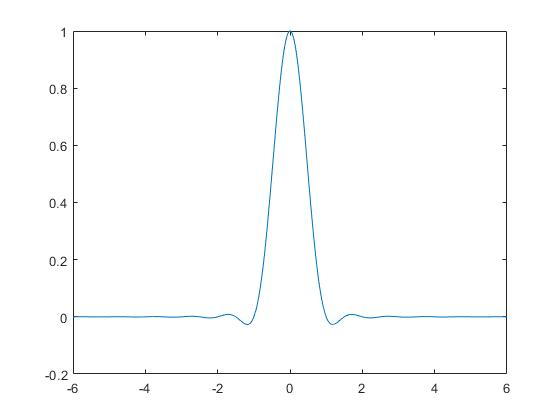
\includegraphics[width = 0.4\linewidth]{Raised_Cosine_Pulse.jpg}
    \caption{Raised Cosine Pulse}
    \label{fig:Raised_Cosine_Pulse}
  \end{center}
\end{figure}
\subsubsection{Triangle Pulse}
\begin{figure}[H]
  \begin{center}
    \begin{subfigure}[b]{0.4\linewidth}
      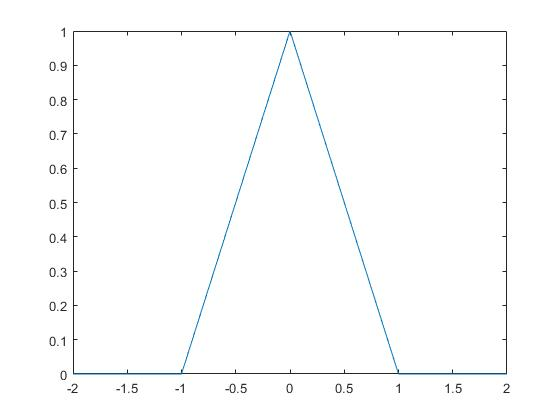
\includegraphics[width = \linewidth]{Tri_Half.jpg}
      \caption{Triangular Half Width Pulse}
    \end{subfigure}
    \begin{subfigure}[b]{0.4\linewidth}
      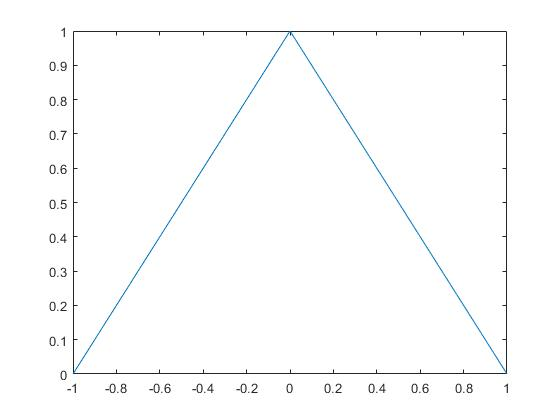
\includegraphics[width = \linewidth]{Tri_Full.jpg}
      \caption{Triangular Full Width Pulse}
    \end{subfigure}
    \caption{Triangular Pulse}
    \label{fig:Tri_Half}
  \end{center}
\end{figure}
\subsubsection{Rectangle Half Width}
\begin{figure}[H]
  \begin{center}
    \begin{subfigure}[b]{0.4\linewidth}
      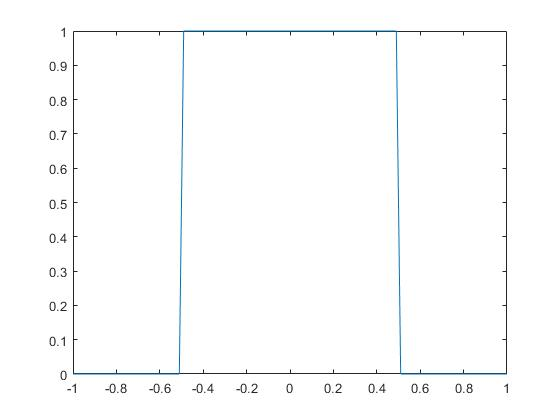
\includegraphics[width = \linewidth]{Rect_Half.jpg}
      \caption{Rectangular Half Width Pulse}
    \end{subfigure}
    \begin{subfigure}[b]{0.4\linewidth}
      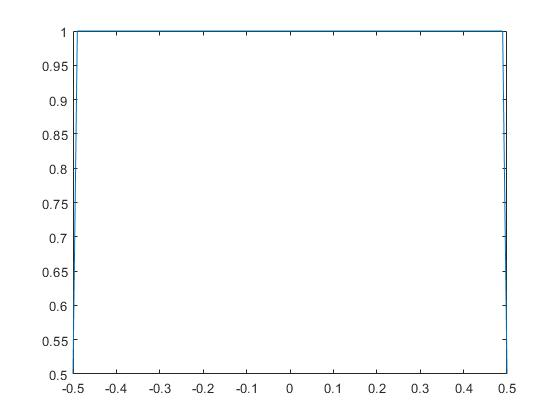
\includegraphics[width = \linewidth]{Rect_Full.jpg}
      \caption{Rectangular Full Width Pulse}
    \end{subfigure}
    \caption{Triangular Pulse}
    \label{fig:Tri_Half}
  \end{center}
\end{figure}
\subsubsection{Sinc}
\begin{figure}[H]
  \begin{center}
    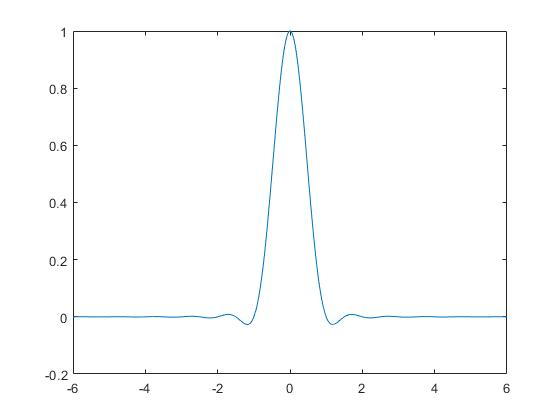
\includegraphics[width = \linewidth]{Raised_Cosine_Pulse.jpg}
    \caption{Raised Cosine Pulse}
    \label{fig:Raised_Cosine_Pulse}
  \end{center}
\end{figure}
\subsubsection{Sinc Squared}
\begin{figure}[H]
  \begin{center}
    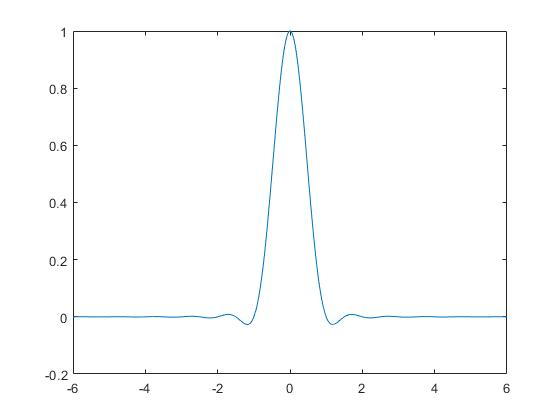
\includegraphics[width = \linewidth]{Raised_Cosine_Pulse.jpg}
    \caption{Raised Cosine Pulse}
    \label{fig:Raised_Cosine_Pulse}
  \end{center}
\end{figure}

\subsection{Sin Pulse}











\section{Results}

\subsection{Polar}

\subsection{On-Off}

\subsection{Bipolar}

\subsection{Duobinary}



\end{document}
